\chapter{Introduction to Natural Language Processing}

\section{Applying Machine Learning to Text}

Text data differs significantly from the numerical or categorical data we have seen so far. It is unstructured, variable in length, and high-dimensional.

\begin{definitionblock}[Text]
A \bfit{text} is a sequence of symbols (characters, words, or sentences) belonging to an alphabet $A$. Formally:
$$
    x \in A^*
$$
where $A^*$ is the set of all possible strings of symbols from $A$ (in modern contexts, usually UTF-16).
\end{definitionblock}

\begin{minipage}{0.45\textwidth}
In NLP terminology:
\begin{itemize}
    \item A single text $x$ is called a \textbf{document}.
    \item A dataset $D$ of texts is called a \textbf{corpus}.
\end{itemize}
\end{minipage}
\hfill
\begin{minipage}{0.53\textwidth}
    \centering
    
\includegraphics[width=0.8\textwidth]{assets/fig39.png}
    \vspace{-0.5em}
    \captionof{figure}{Text-to-vector transformation pipeline.}
\end{minipage}

\begin{exampleblock}[Sentiment Analysis]

A classic application is \textbf{Sentiment Analysis}. The goal is to gain insights about the sentiments an author was feeling while writing a document.
This is a standard \textbf{supervised learning problem}:
\begin{itemize}
    \item Input $X$: A set of documents (strings).
    \item Output $Y$: A sentiment label (e.g., $Y = \{\text{Positive}, \text{Negative}, \text{Neutral}\}$).
\end{itemize}
\end{exampleblock}

Since standard ML models (SVM, Random Forest, etc.) require numerical vectors as input, a \textbf{text-to-vector} transformation $f_{\text{text-to-vect}}$ is essential to obtain multivariate observations $x' \in \mathbb{R}^p$.

\subsection{Feature Engineering: From Text to Vectors}
\subsubsection{Common Text Pre-processing Steps}

Each preprocessing step is a function $f_{\text{pre-proc}}: A^* \to A^*$:
\begin{itemize}
    \item \textbf{Case conversion}: everything to lowercase (language independent). E.g., $x = \text{``Banana is my favorite fruit''} \mapsto x' = \text{``banana is my favorite fruit''}$.
    \item \textbf{Removal of punctuation}: (language independent).
    \item \textbf{Stemming}: each word is replaced with its morphological root (language dependent). E.g., $x = \text{``I liked eating bananas''} \mapsto x' = \text{``I lik eat banana''}$.
    \item \textbf{Removal of stop-words}: (language dependent). Stop words are very common words (articles, some prepositions, etc.).
\end{itemize}
\subsubsection{Bag of Words (BoW)}

\textbf{Bag-of-words} (BoW) is a $f_{\text{text-to-vect}}$ based on the idea of associating one numerical variable with each word in a predefined dictionary $W \in \mathcal{P}(A^*)$. Formally, $f_{\text{BOW}}$ maps $x \in A^*$ to $x' \in \mathbb{R}^{|W|}$, taking the dictionary $W$ as a parameter. Given $W$ and a document $x \in A^*$:
\begin{enumerate}
    \item \textbf{Tokenize} $x$ into a multiset $T = f_{\text{tokenize}}(x)$ of tokens (words).
    \item For each $t \in T$, set $x'_t$ to the multiplicity $m(t, T)$ of $t$ in $T$, i.e., to the number of occurrences of $t$ in $x$.
\end{enumerate}
The outcome is $x' \in \mathbb{R}^{|W|}$. An alternative is to use frequencies instead of raw counts: $x'_t = \frac{m(t, T)}{|T|}$, which is useful when documents have very different lengths but length itself is not relevant.

BoW considers slightly different sequences of characters as different words (and hence as different features) because of tokenization; usually this is undesirable. 

\begin{figure}[H]
    \centering
    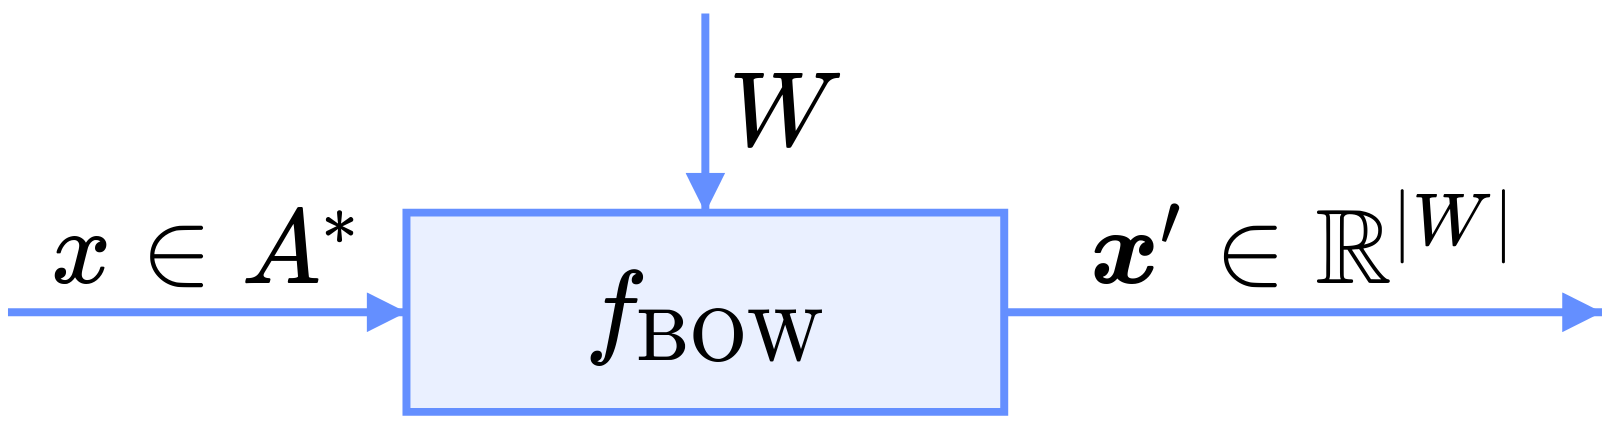
\includegraphics[width=0.4\textwidth]{assets/bow.png}
    \vspace{-0.5em}
    \caption{The Bag of Words representation.}
\end{figure}

\subsubsection{TF-IDF}

A major limitation of simple BoW counting is that it tends to highlight words that are very frequent in the corpus but not necessarily informative (e.g., ``good'' might appear in almost every review).

To address this, we use \textbf{TF-IDF} (Term Frequency-Inverse Document Frequency). It weighs a word by how important it is to a specific document within the entire corpus.

$$
\text{tfidf}(t, d, D) = \text{tf}(t, d) \cdot \text{idf}(t, D)
$$

Where:

\begin{minipage}{0.53\textwidth}
\begin{itemize}
    \item $t$ is the term (word);
    \item $d$ is the specific document;
    \item $D$ is the corpus (collection of all documents);
    \item $\text{tf}(t, d)$ is the \textbf{Term Frequency}: \\
    frequency of term $t$ in document $d$ (often normalized).
    \item $\text{idf}(t, D)$ is the \textbf{Inverse Document Frequency}:
    $$
    \text{idf}(t, D) = \log \left( \frac{|D|}{|\{d \in D : t \in d\}|} \right)
    $$
\end{itemize}
\end{minipage}%
\hfill
\begin{minipage}{0.45\textwidth}
    \centering
    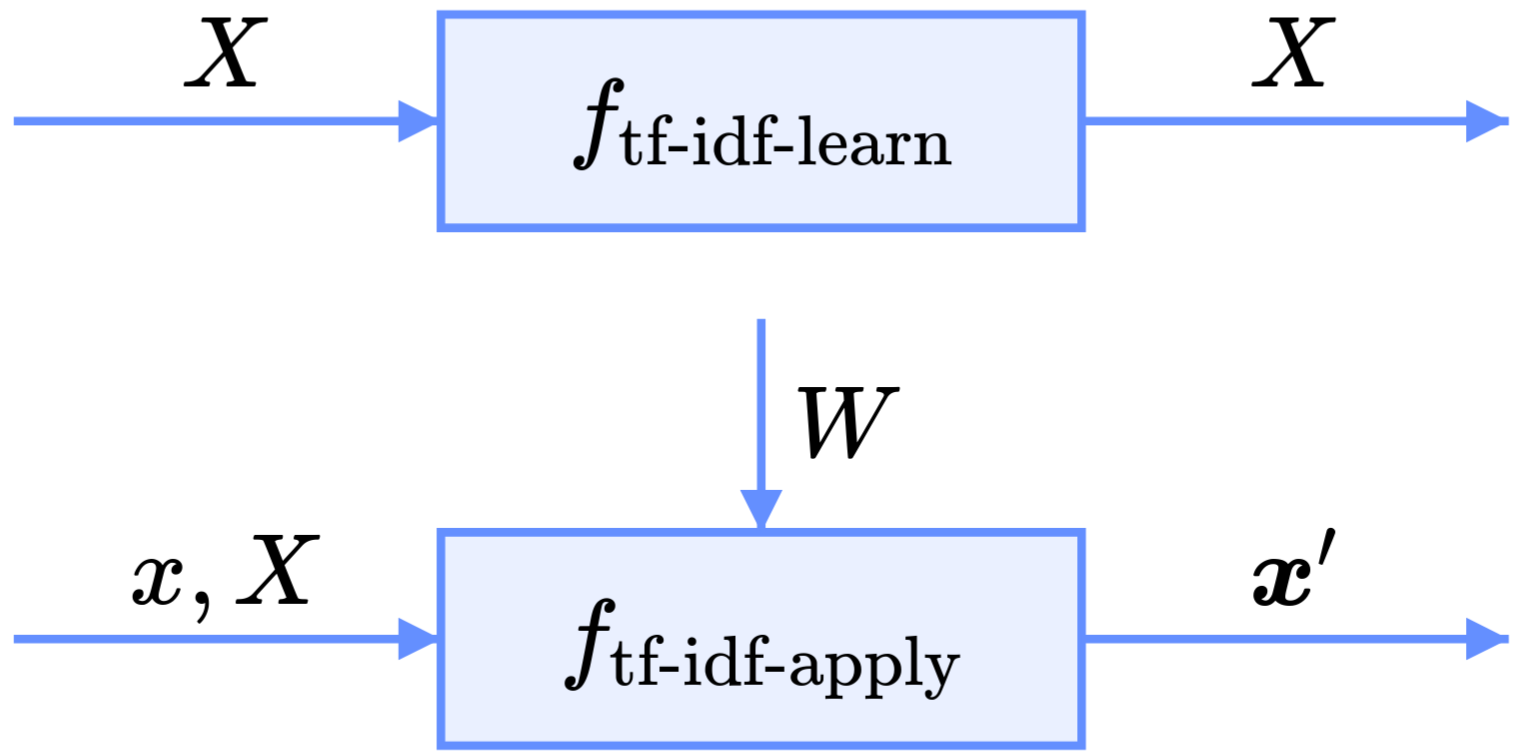
\includegraphics[width=0.95\textwidth]{assets/tf-idf.png}
    \captionof{figure}{The TF-IDF representation.}
\end{minipage}

\begin{itemize}
\item[] It measures how rare the term is across the corpus.
\end{itemize}

\begin{tipsblock}[Intuition]
    \begin{itemize}
        \item High TF: The word appears often in this document.
        \item High IDF: The word is rare in the corpus (informative).
        \item \textbf{High TF-IDF}: The word is frequent in \textit{this} document but rare elsewhere $\to$ it characterizes the document well.
    \end{itemize}
\end{tipsblock}

\subsubsection{Dimensionality and Context}

With $f_{\text{BOW}}$, the output dimension is $p = |W|$, which can be huge. Common reduction practices include:
\begin{itemize}
    \item Using a very small, domain-specific dictionary.
    \item Learning the dictionary from data (e.g., keeping only the top-$k$ most frequent words).
    \item Using dimensionality reduction techniques (e.g., PCA/SVD) on the resulting matrix.
\end{itemize}

\textbf{The problem of Ordering}:
BoW destroys word order (``not bad'' becomes ``bad'' + ``not'', losing the negation context). To capture context, we can use:
\begin{itemize}
    \item \textbf{N-grams}: Instead of counting single words ($1$-grams), we count sequences of $n$ adjacent words (e.g., $2$-grams like ``not bad'', ``very good''). This drastically increases dimensionality.
    \item \textbf{Part of Speech (POS) Tagging}: Analyzing the grammatical role (noun, verb, adjective) of words to disambiguate meaning (e.g., ``book'' as a noun vs.\ ``book'' as a verb).
\end{itemize}
